% *********************************************************************
% © 2016–2025 Jeremy Sylvestre
%
% Permission is granted to copy, distribute and/or modify this document
% under the terms of the GNU Free Documentation License, Version 1.3 or
% any later version published by the Free Software Foundation; with no
% Invariant Sections, no Front-Cover Texts, and no Back-Cover Texts. A
% copy of the license is included in the appendix entitled “GNU Free
% Documentation License” that appears in the output document of this
% PreTeXt source code. All trademarks™ are the registered® marks of
% their respective owners.
%
% *********************************************************************
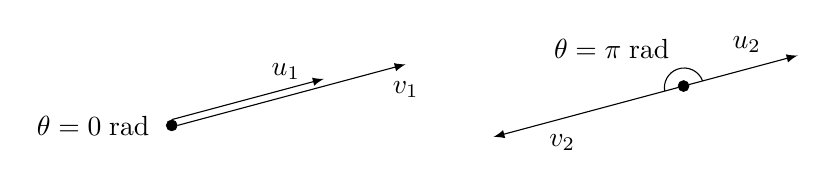
\begin{tikzpicture}[
	point/.style={circle,draw,very thin,fill,inner sep=0pt,minimum size=4pt},
	vector/.style={-latex},
]
	\node[point] at (0,0) (o) {};
	\draw[vector] (o.north) to node[above,near end] {$\uvec{u}_1$} ++(15:2cm);
	\draw[vector] (o.east) to node[below,at end,yshift=-0.1cm] {$\uvec{v}_1$} ++(15:3cm);
	\node at (-1,0) {$\theta = 0\;\mathrm{rad}$};
	\begin{scope}[xshift=6.5cm,yshift=0.5cm]
		\node[point] at (0,0) (o) {};
		\draw[vector] (o) to node[above left, near end] {$\uvec{u}_2$} ++(15:1.5cm);
		\draw[vector] (o) to node[below right,near end] {$\uvec{v}_2$} ++(195:2.5cm);
		%	\node at (0.5,0) {$\theta = \pi\;\mathrm{rad}$};
		\draw (0,0) ++(15:0.25cm) arc (20:190:0.25cm) node[above left,midway]
			{$\theta = \pi\;\mathrm{rad}$};
	\end{scope}
\end{tikzpicture}
